\section{Evaluation}

The dataset is devided into training dataset and test dataset. Training dataset includes 80\% (299 earthquakes) of total dataset and test dataset includes 20\% (75 earthquakes) of total dataset. We trained the model 50 steps and shuffled training dataset in each steps to prevent overfitting.

%%%

Figure ~\ref{fig:arrival_loss_10} shows the loss of S-wave arrival time with 10 fast earthquake arrived seismic stations.

\begin{figure}[t]
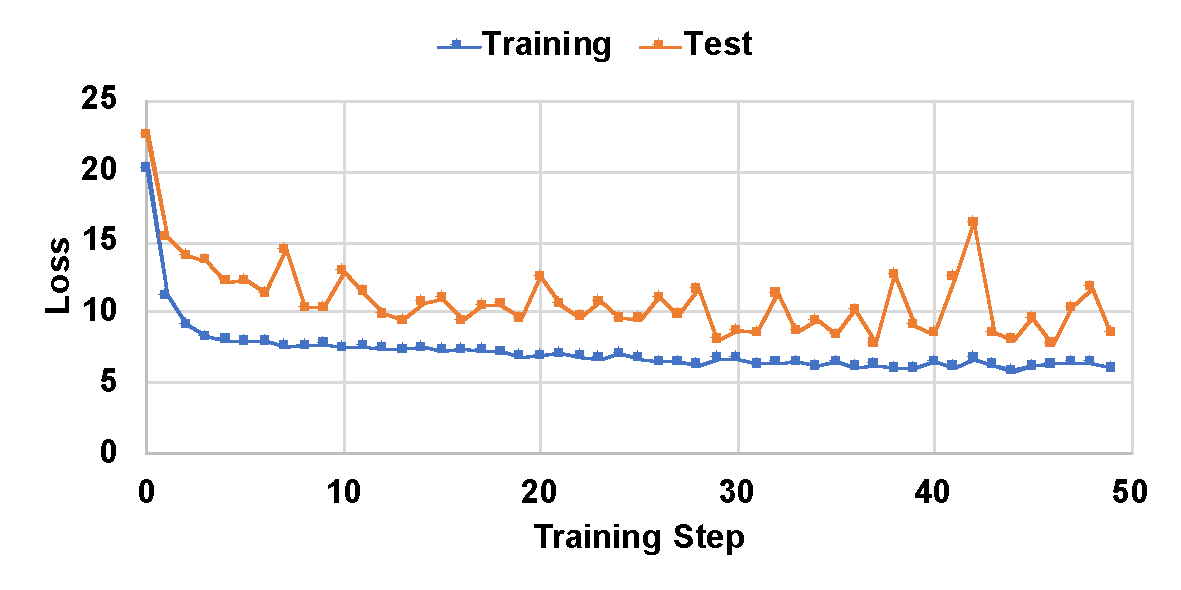
\includegraphics[width=0.48\textwidth]{figs/arrival_loss_10.pdf}
\caption{Loss of arrival time estimation with 10 seismic stations}
\label{fig:arrival_loss_10}
\end{figure}

Figure ~\ref{fig:center_loss_10} shows the loss of location of hypocenter with 10 fast earthquake arrived seismic stations.

\begin{figure}[t]
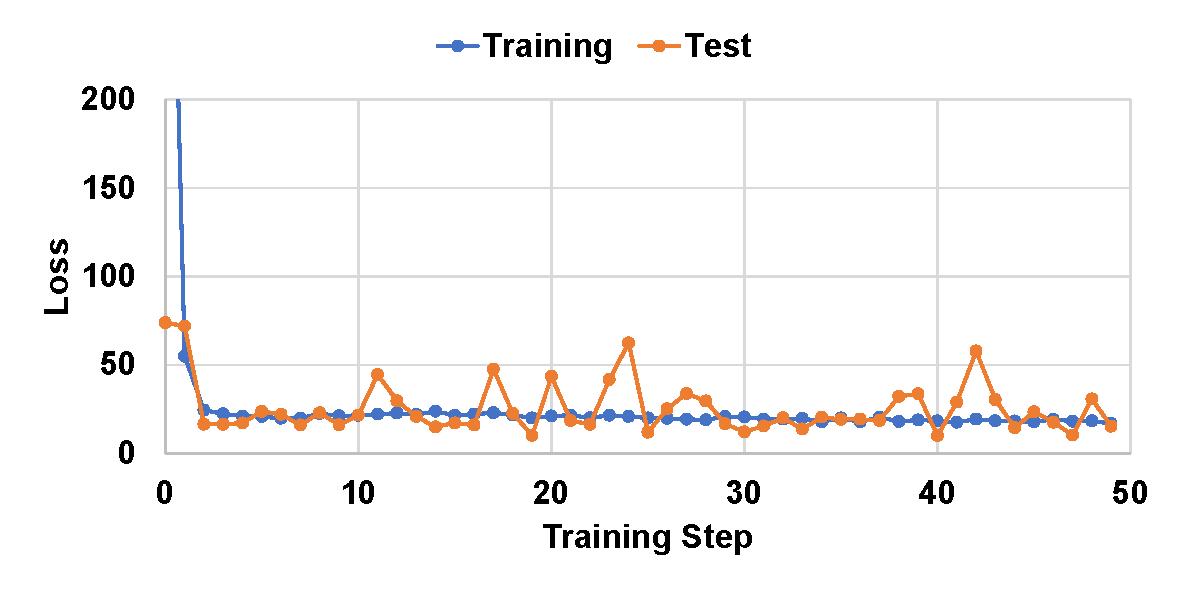
\includegraphics[width=0.48\textwidth]{figs/center_loss_10.pdf}
\caption{Loss of hypocenter estimation with 10 seismic stations}
\label{fig:center_loss_10}
\end{figure}

Figure ~\ref{fig:mag_loss_10} shows the loss of magnitude with 10 fast earthquake arrived seismic stations.

\begin{figure}[t]
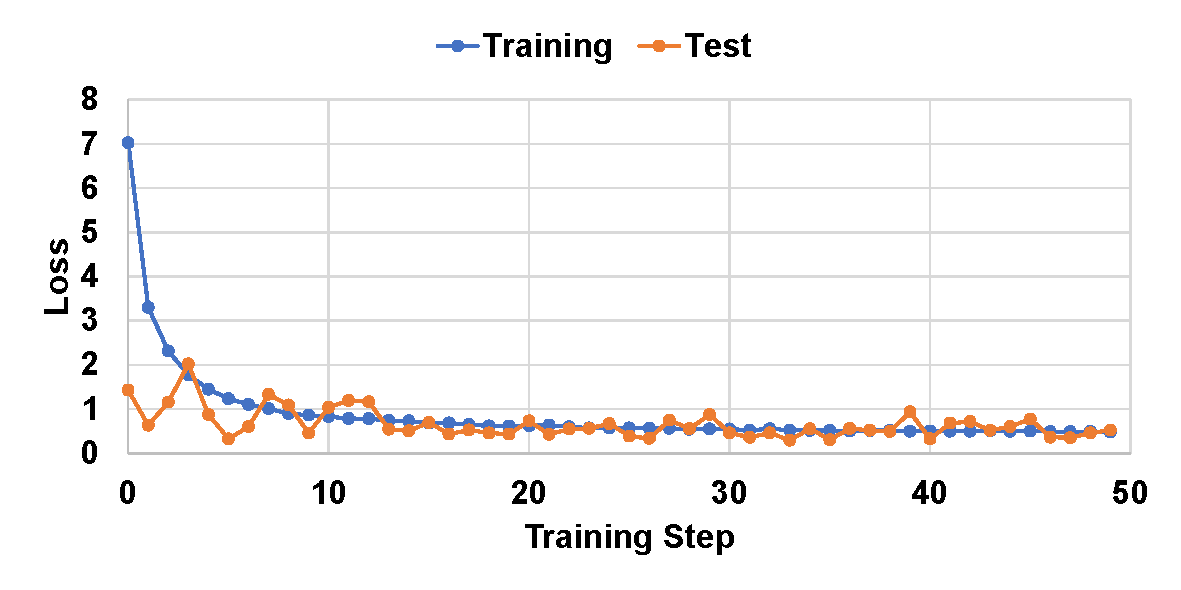
\includegraphics[width=0.48\textwidth]{figs/mag_loss_10.pdf}
\caption{Loss of magnitude prediction with 10 seismic stations}
\label{fig:mag_loss_10}
\end{figure}

%%%

Figure ~\ref{fig:center_loss_3} shows the loss of S-wave arrival time with 3 fast earthquake arrived seismic stations.

\begin{figure}[t]
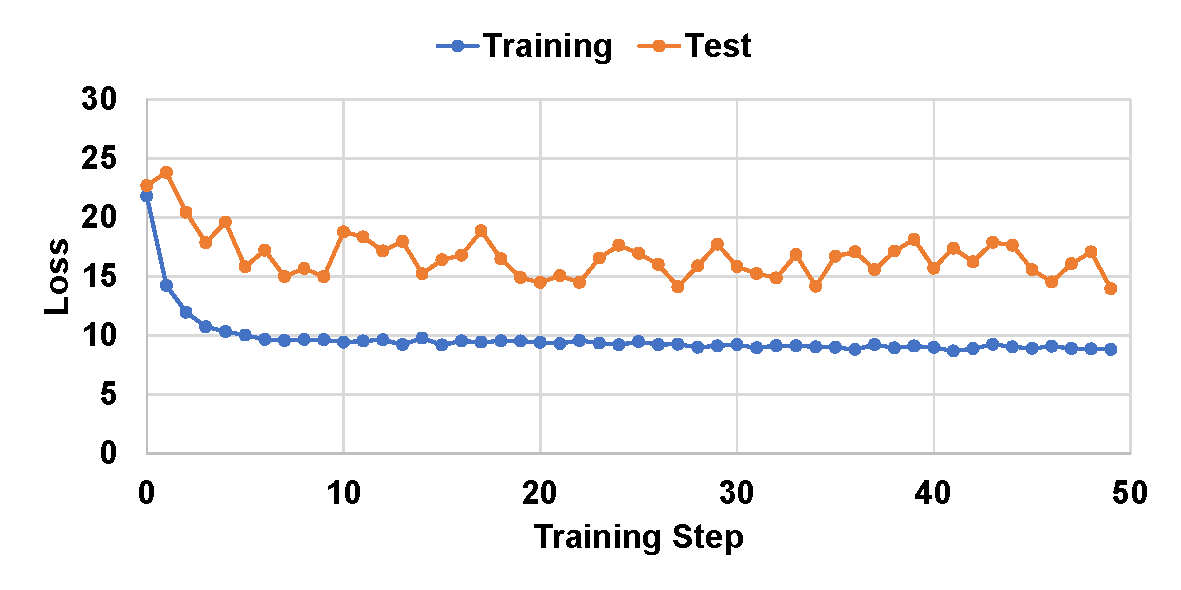
\includegraphics[width=0.48\textwidth]{figs/arrival_loss_3.pdf}
\caption{Loss of arrival time estimation with 3 seismic stations}
\label{fig:arrival_loss_3}
\end{figure}

Figure ~\ref{fig:center_loss_3} shows the loss of location of hypocenter with 3 fast earthquake arrived seismic stations.

\begin{figure}[t]
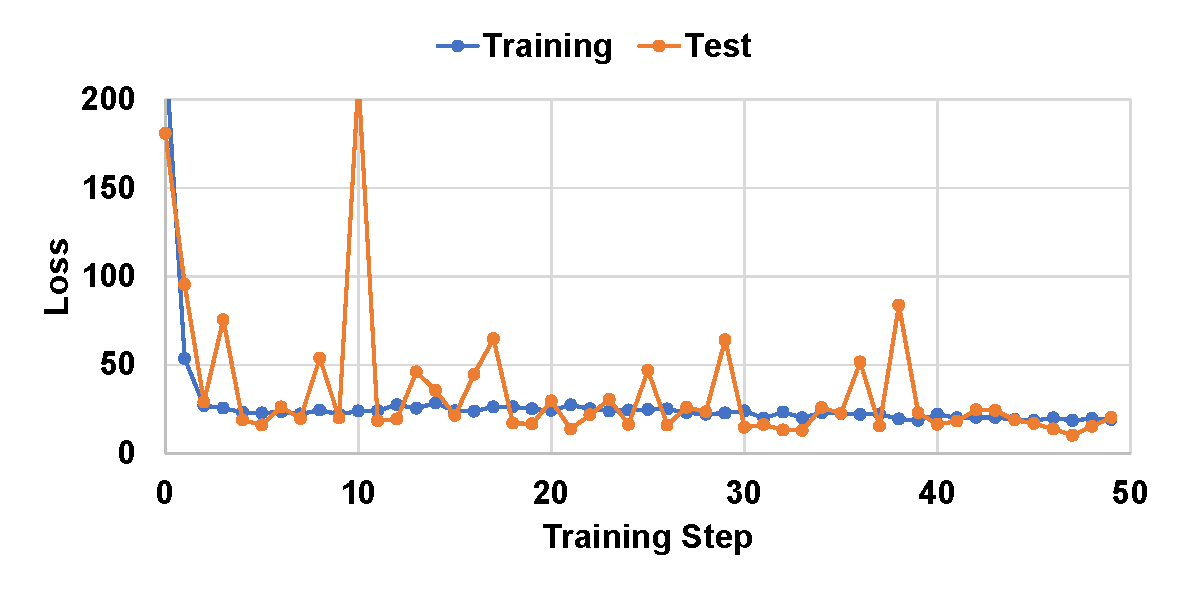
\includegraphics[width=0.48\textwidth]{figs/center_loss_3.pdf}
\caption{Loss of hypocenter estimation with 3 seismic stations}
\label{fig:center_loss_3}
\end{figure}

Figure ~\ref{fig:mag_loss_3} shows the loss of magnitude with 3 fast earthquake arrived seismic stations.

\begin{figure}[t]
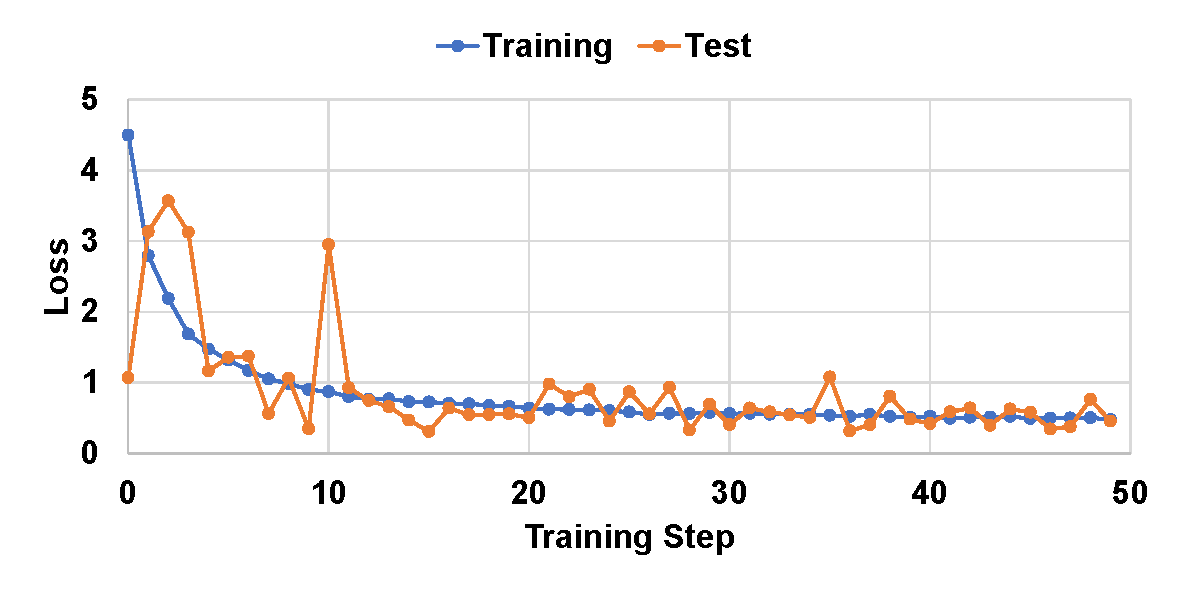
\includegraphics[width=0.48\textwidth]{figs/mag_loss_3.pdf}
\caption{Loss of magnitude prediction with 3 seismic stations}
\label{fig:mag_loss_3}
\end{figure}

%%%

Figure ~\ref{fig:arrival_loss_1} shows the loss of S-wave arrival time with the fastest earthquake arrived seismic stations.

\begin{figure}[t]
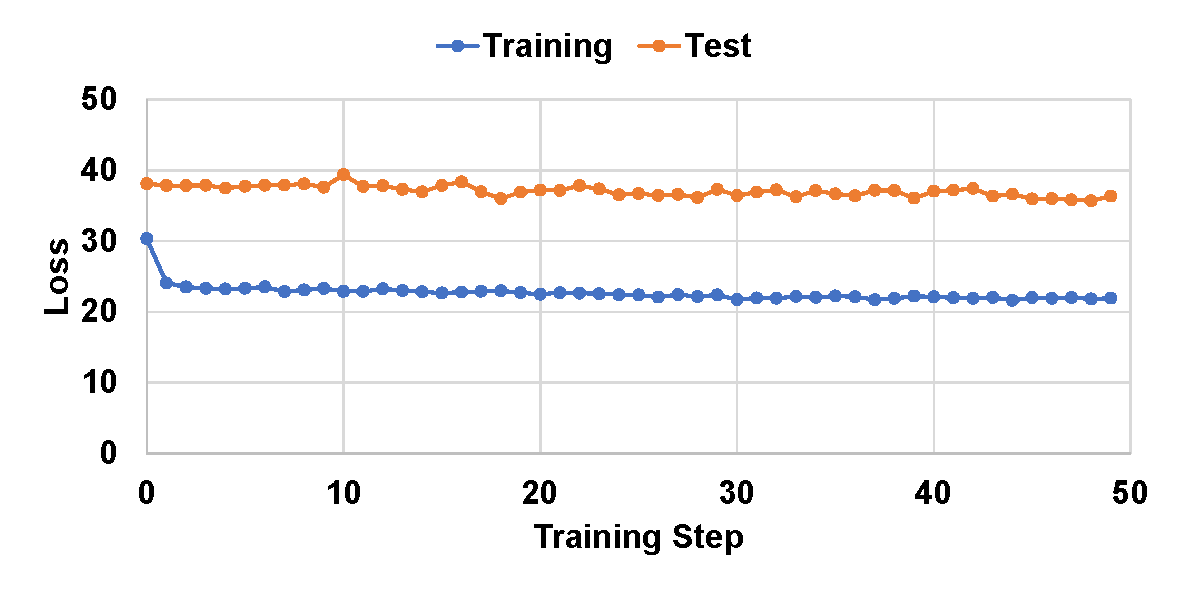
\includegraphics[width=0.48\textwidth]{figs/arrival_loss_1.pdf}
\caption{Loss of arrival time estimation with the fastest seismic stations}
\label{fig:arrival_loss_1}
\end{figure}

Figure ~\ref{fig:center_loss_1} shows the loss of location of hypocenter with the fastest earthquake arrived seismic stations.

\begin{figure}[t]
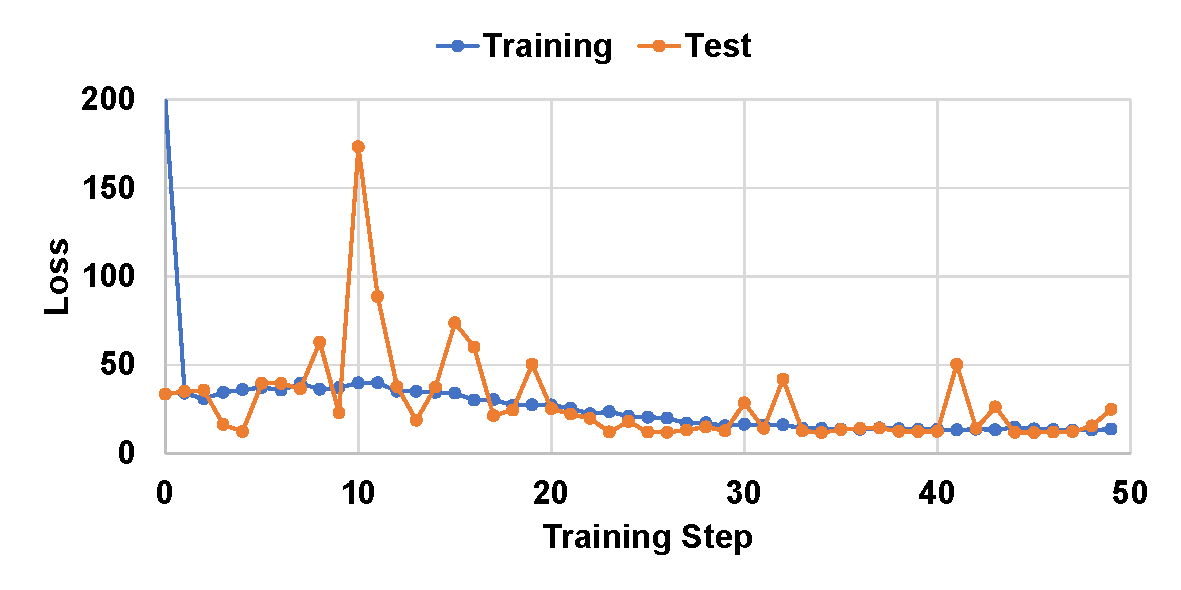
\includegraphics[width=0.48\textwidth]{figs/center_loss_1.pdf}
\caption{Loss of hypocenter estimation with the fastest seismic stations}
\label{fig:center_loss_1}
\end{figure}

Figure ~\ref{fig:mag_loss_1} shows the loss of magnitude with the fastest earthquake arrived seismic stations.

\begin{figure}[t]
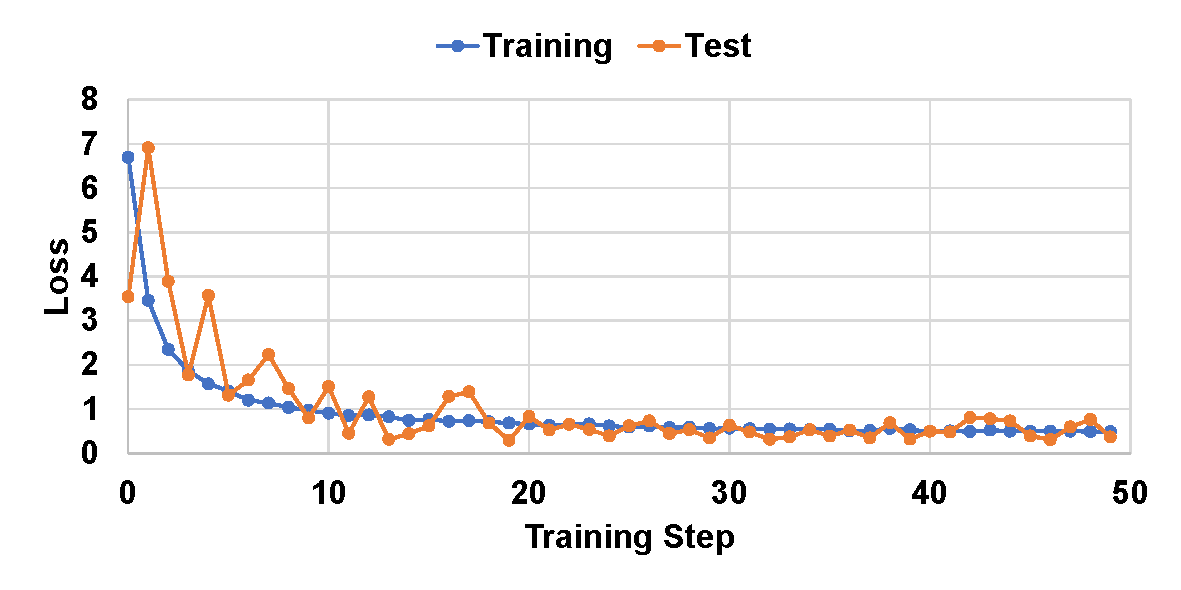
\includegraphics[width=0.48\textwidth]{figs/mag_loss_1.pdf}
\caption{Loss of magnitude prediction with the fastest seismic stations}
\label{fig:mag_loss_1}
\end{figure}

%%%

Figure ~\ref{fig:arrival_each} shows the S-wave arrival time loss of each seismic stations with the 10 fast earthquake arrived seismic stations.

\begin{figure}[t]
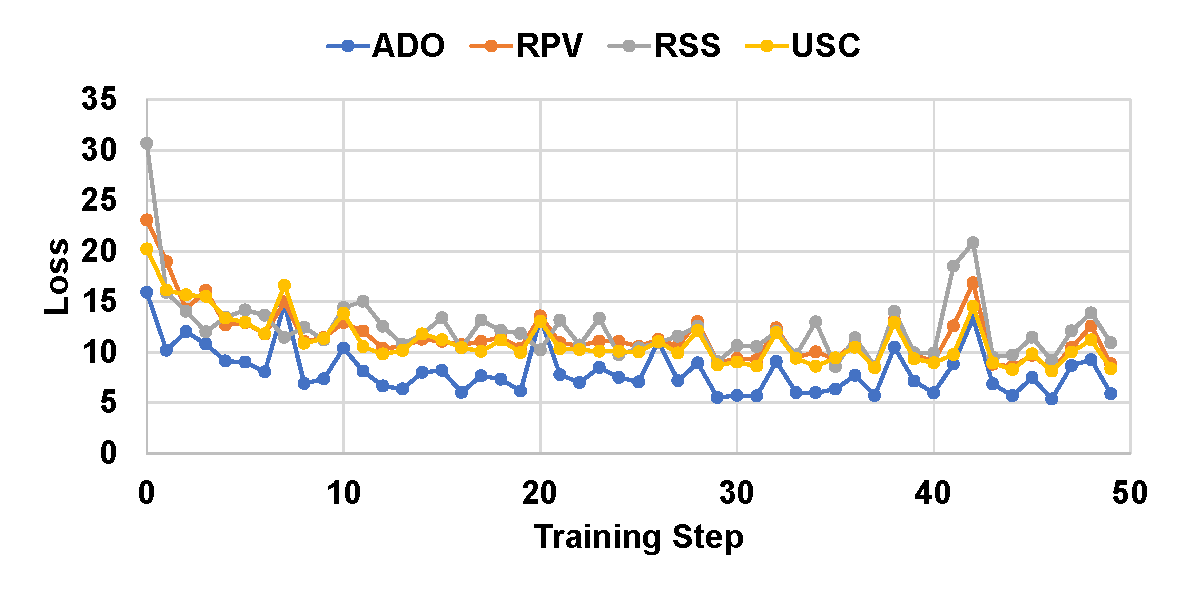
\includegraphics[width=0.48\textwidth]{figs/arrival_loss_detail_10.pdf}
\caption{S-wave arrival time loss of each seismic stations (i.e., ADO, RPV, RSS and USC) with 10 seismic stations}
\label{fig:arrival_each}
\end{figure}

Figure ~\ref{fig:center_each} shows the loss of latitude, longitude and depth with the 10 fast earthquake arrived seismic stations.

\begin{figure}[t]
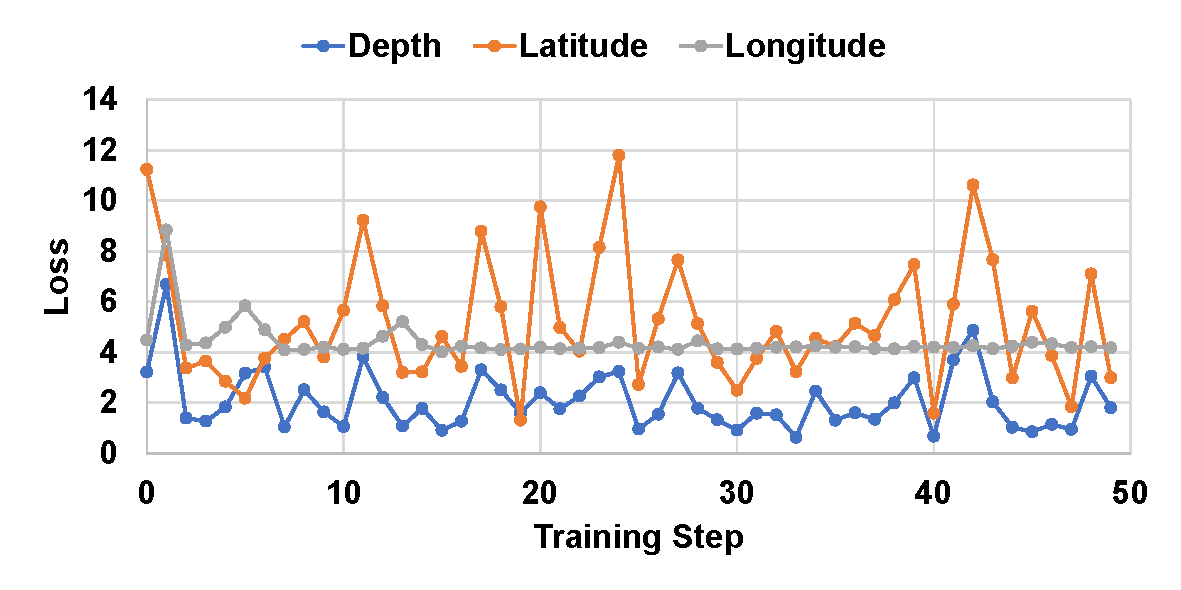
\includegraphics[width=0.48\textwidth]{figs/center_loss_detail_10.pdf}
\caption{latitude, longitude and depth loss with 10 seismic stations}
\label{fig:center_each}
\end{figure}

%%%
